\documentclass[a4paper,11pt]{article}
\usepackage[T1]{fontenc}
\usepackage[utf8]{inputenc}
\usepackage{lmodern}
\usepackage[top=2cm, bottom=2cm, left=2cm, right=2cm]{geometry}
\usepackage{graphicx}
\usepackage{listings}
\usepackage{color}

\title{Implementation of a compiler for an imperative language\\IMP}
\author{Remy Detobel \& Denis Hoornaert}
 
\definecolor{codegreen}{rgb}{0,0.6,0}
\definecolor{codegray}{rgb}{0.5,0.5,0.5}
\definecolor{codepurple}{rgb}{0.58,0,0.82}
\definecolor{backcolour}{rgb}{0.95,0.95,0.92}
 
\lstdefinestyle{mystyle}{
    backgroundcolor=\color{backcolour},   
    commentstyle=\color{codegreen},
    keywordstyle=\color{magenta},
    numberstyle=\tiny\color{codegray},
    stringstyle=\color{codepurple},
    basicstyle=\footnotesize,
    breakatwhitespace=false,         
    breaklines=true,                 
    captionpos=b,                    
    keepspaces=true,                 
    numbers=left,                    
    numbersep=5pt,                  
    showspaces=false,                
    showstringspaces=false,
    showtabs=false,                  
    tabsize=2
}
 
\lstset{style=mystyle}

\begin{document}

\maketitle

\section{Introduction}

  The project aim is to implement a compiler for a 'simple' imperative language named \textit{IMP}. Like any imperative programming language, \textit{IMP} is structured of mainstream features such as \textit{keywords} (\verb|if|, \verb|while|, ... statements), \textit{variables}, \textit{numbers} and \textit{comments}.
  The form of these features follows some defined rules~:
  \begin{itemize}
    \item a \textit{variable} is a sequence of alphanumeric characters that must start by a letter.
    \item a \textit{number} is a sequence of one or more digits.
    \item a \textit{comment} must start by the combination '\verb|(*|' and ends by the reversed combination '\verb|*)|'. 
  \end{itemize}
  The compilation scheme is generally divided in three main phases~: analysis, synthesis and optimization. The phases are themselves composed of different steps. For instance, the analysis phase is composed of \textit{lexical analysing} step (or \textit{scanning}), a \textit{syntax analysing} step (or \textit{parsing}) and a \textit{semantic analysing} step. In this assignment, the focus is set on the \textit{analysis phase}.
  \begin{figure}[h]
      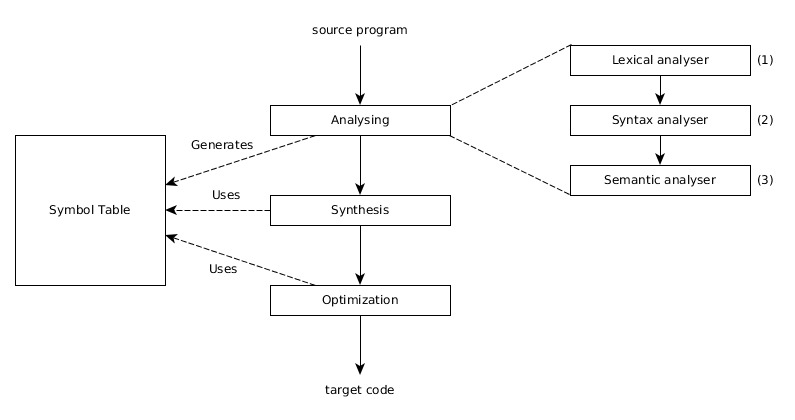
\includegraphics[scale=0.5]{./img/phase_of_compiler.jpg}
      \centering
      \caption{Compilation phases}
    \end{figure}
  
\section{Implementation of the lexical analyser}

  In the so called "Dragon book"\footnote{V. Aho, A., 2007. \textit{Compilers~: Principles, techniques, \& Tools.} 2nd ed. New York~: Pearson.} the \textit{lexical anlyser} is defined as follow~:
  \begin{center}
    <<The \textit{lexical analyser} reads the stream of characters making up the source program and groups the character into a meaningful sequence called \textit{lexemes}.>>
  \end{center}
  A \textit{lexeme} can be defined as a tuple which contains both a \textit{token name} and the associated value (not always mandatory). The sequence of \textit{lexemes} generated by the \textit{lexical analyser} will be used by the following step. In addition, the \textit{lexical analyser} will generate a very useful tool, that will be used by all the other steps (as shown in fig 1.), called a \textit{symbol table}. The role of the \textit{symbol table} is to store every variable encountered while scanning the source code and the line where it appears for the first time.\\
  
  \subsection{The use of a lexical analyser generator}
    In order to ease the process of recognizing the lexemes defined in the given \verb|LexicalUnits.java| many \textit{lexical analysers} bave been develloped. Among them, the most well known generator is the flex program and all its derived versions. In the present project, \verb|jflex| is used as it has been decided to implement the project using the \verb|java| programming language. Using a \textit{lexical analyser generator} eases the analysis of any input because it enables the programmers to describe every \textit{regular expression} by using the \textit{Regex} writing convention and then to generate a \verb|.java| file that will recognise all of them. This generated \verb|.java| file can then be used as any other \verb|java| class. 
  
  \subsection{Lexical analyser structure}
    \begin{figure}[h]
      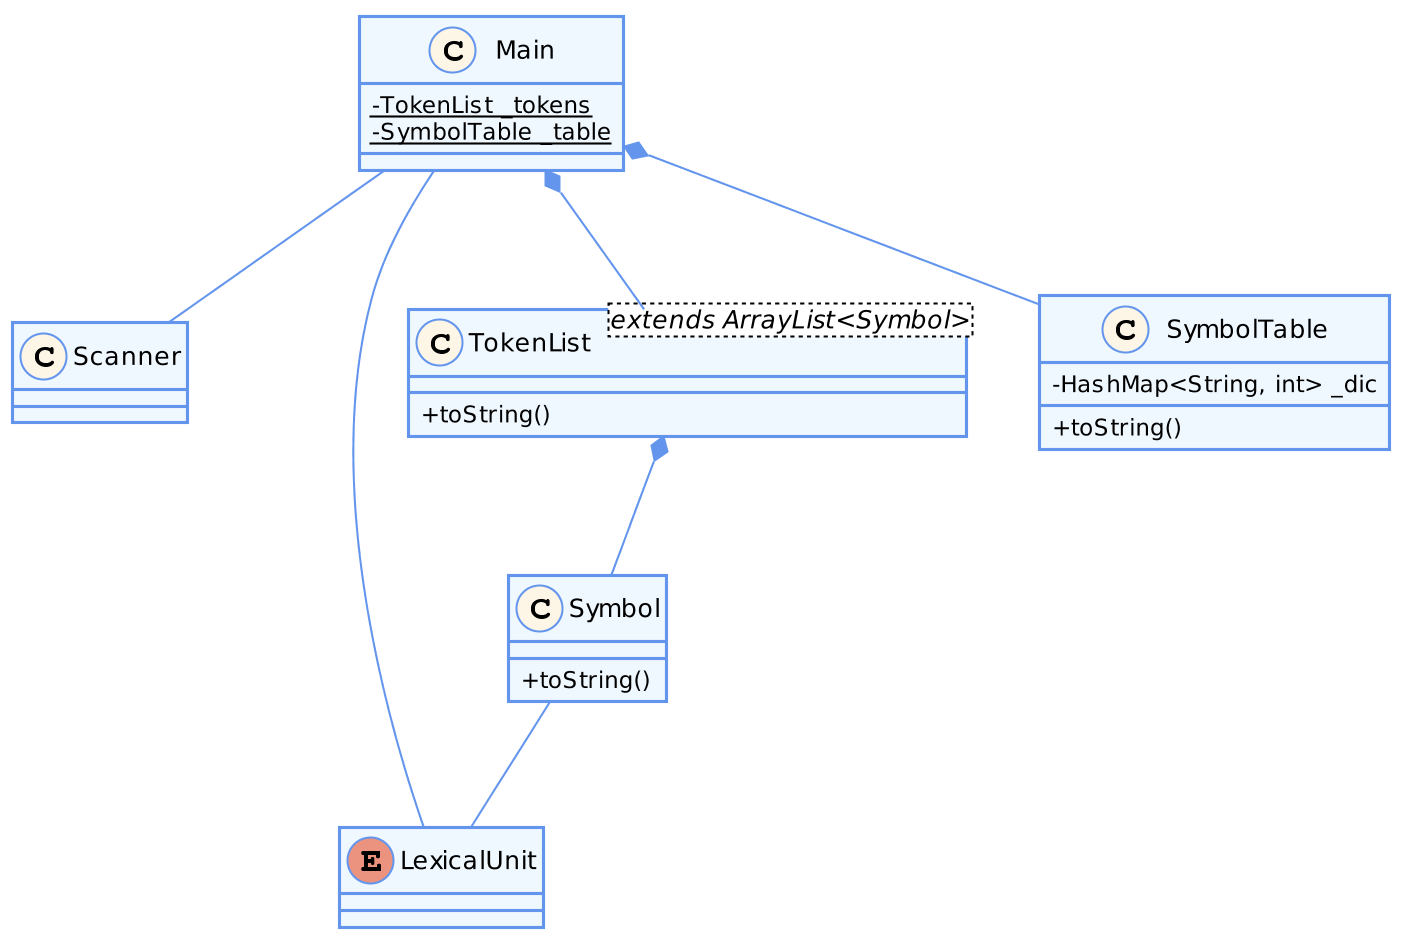
\includegraphics[scale=0.25]{./img/class_diag.png}
      \centering
      \caption{Model class}
    \end{figure}
  
  \subsection{Regular expressions}

  \subsection{Dealing with nested comments}
    The management of comments using regular language is quite simple. Once an opening statement (here : \verb|(*|) has been encountered, it overlooks the following characters until it encounters a closing statement (here : \verb|*)|).
    \begin{lstlisting}
(*I am a (*nested*) comment*)
    \end{lstlisting}
    Unfortunately, applying the same mechanism on a nested comment will result in a ill-formed outcome. Indeed, in the case of the example above, the analyser will overlook the second opening statement (columns 9 \& 10) and will stop when it comes across the first closing statement (columns 17 \& 18) having for consequence that the third part of the \textit{nested comment} will remain.\\
    To overcome this problem, the analyser must know how many opening statement it came across and how many closing statement it should expect to encounter in order to know whether it is still in a comment.\\
    The most obvious and smartest way to implement it is to use a counter (i.e. a memory) that will be incremented for every opening statement encountered and decreased for every closing statement encountered. However, from a theoretical point of view, by using a memory the language cannot be considered as regular any more. In the present project, it is not a problem and \verb|jflex| allows us to implement such a language.
    % Remy: peut-être rajouter un mot également sur le fait que un commentaire imbriqué n'a pas de sens réel vu qu'on ignore tout ce qui n'est pas une fermeture de commentaire dans un commentaire ;)
    
  \subsection{Tests}
    
    \lstinputlisting{../test/Euclid.imp}
    \lstinputlisting{../test/Search.imp}
    \lstinputlisting{../test/Sort.imp}

\section{How to set up the project}
  In order to simplify the compilation and the support of external libraries, it has been decided to use a well known \textit{java} project manager named \textit{Maven}. Its configuration file (\verb|pom.xml|) defines the \verb|main| file, defines the source folder, the \textit{JFlex} library and the package that must be compiled with this library.
  % denis : source folder or folders ?
  % denis : "the \textit{JFlex} library" no verb ? you mean "manages the \textit{JFlex} library" ?
  \subsection{Compilation}
    Compiling the project with \textit{Maven} is easy as the user only needs to execute~: \verb|mvn clean compile|. However, at the first execution, the user needs to execute \verb|mvn install| so that \textit{Maven} can install the library.\\ % denis : il y a une ou plusieurs librairies ?
    If the user does not want to use \textit{Maven}, he can execute different commands from the root project~:
    \begin{verbatim}
java -jar jflex-1.6.1.jar -d src/be/ac/ulb/infof403/ src/be/ac/ulb/infof403/lex/Scanner.flex
    \end{verbatim}
    Where \verb|jflex-1.6.1.jar| is the path to the ``jar'' executable library,  ``-d'' is the output folder path specifier and the last parameter is the path to the ``flex`` file.\\
    Then, the user can compile the java source codes and can create the corresponding ''class`` files. The bash command to compile all the \textit{java} files located in the ''src`` folder is the following~: % denis : J'ai modifié la phrase mais je ne suis aps sur d'avoir compris ce que tu voulais dire.
    \begin{verbatim}
javac -d target $(find ./src/* | grep .java)
    \end{verbatim}
    This command generates the corresponding ''.class`` files and put them in the ''target`` folder. If this folder does not exist at this moment it will then be created. Finally, the ''jar`` file can be generated by using the command~:
    \begin{verbatim}
jar cvfe dist/INFO-F403-IMP.jar be/ac/ulb/infof403/Main -C target/ .
    \end{verbatim}
    Where ''INFO-F403-IMP.jar`` is the name of the generated ''jar`` file and ''target`` is the folder where are located the ''.class`` files.
    
  \subsection{Execution}
    To execute the resulting jar file, the user only has to type~:
    \begin{verbatim}
java -jar dist/INFO-F403-IMP.jar <sourceFile>
    \end{verbatim}
    Where ''sourceFile`` is the path to the IMP file. If the source file is not specified then the program will use the file \verb|test/Euclid.imp|.
    
  \subsection{Test}
    The program has a system which automatically compares each output file (\verb|.out|) to the result of the execution of the corresponding \verb|.imp| file. The execution of the test can be specified by adding the parameter \verb|-test| at the program execution instruction, like this~:
    \begin{verbatim}
java -jar dist/INFO-F403-IMP.jar <sourceFile> -test <testFile>
    \end{verbatim}
    Where ''testFile`` is the name of the output file. If not specified, the program will automatically load a file test based on the ''source file`` name. It will only change the file extension from \verb|.imp| to \verb|.out|.
    

\end{document}
